\chapter*{Výsledky}

\par Na všechny datasety zmíněné v kapitole \emph{Implementace} byly aplikovány algoritmy pro detekci hlavních směrů budovy. Níže jsou detailněji popsány výsledky jednotlivých algoritmů a slovně zhodnoceny výsledné generalizace.

\section*{Dataset Vinohrady}

\par Hustě zastavěná oblast Vinohrad obsahuje mnoho bloků budov, které na sebe plynule navazují. Půdorysy budov jsou především obdélníkového tvaru. Půdorysy některých budov, jako je např. bazilika sv. Ludmily (dole vlevo na jednotlivých oknech \emph{Obrázku 12}), jsou však složitější a nepravidelné.


\begin{figure}[h]
\centering
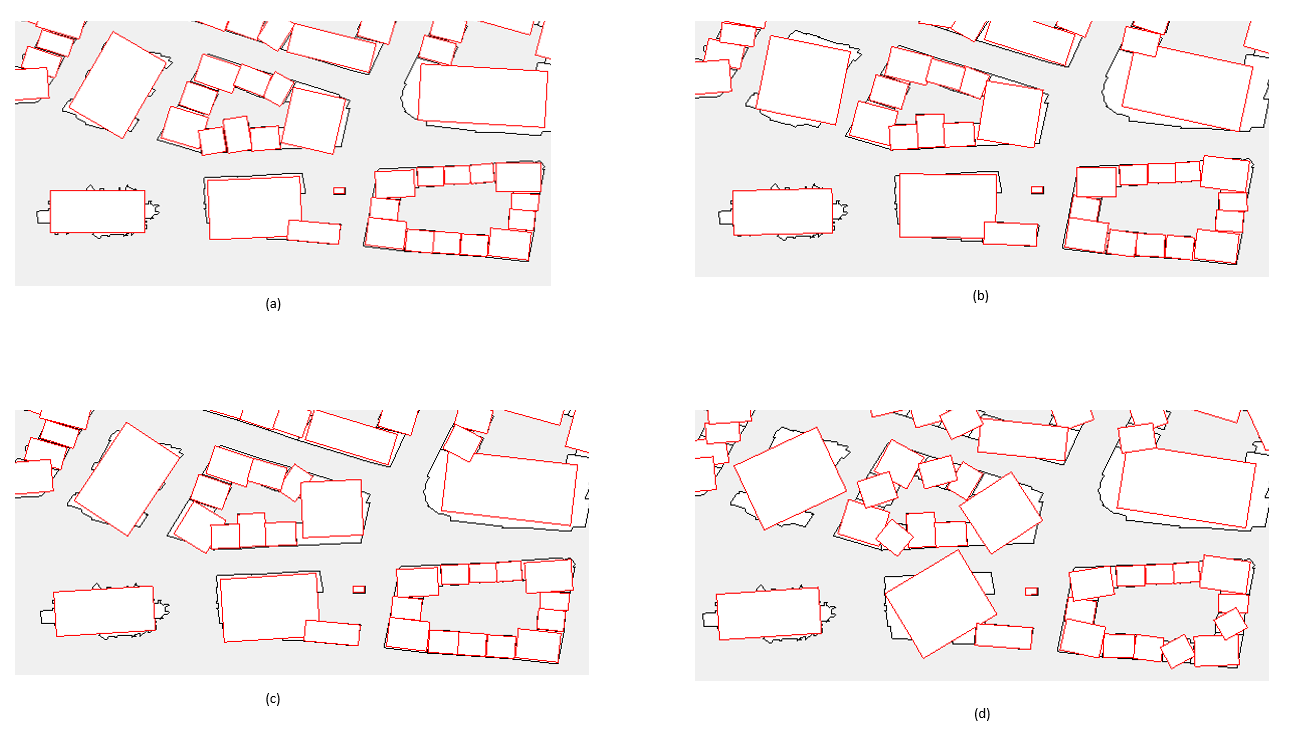
\includegraphics[width=17cm]{vinohrady_porovnani.png}
    \caption{Porovnání generalizačních algoritmů pro Vinohrady. Algoritmy: (a) \emph{MAER}, (b) \emph{Wall Average}, (c) \emph{Longest Edge} a (d) \emph{Weighted Bisector}. (vlastní zpracování).}
\end{figure}

\par Vzhledem na tvar většiny půdorysů dokázala většina algoritmů poměrně přesně určit hlavní směr budovy. Pro tento dataset vystihl hlavní směr budov nejpřesněji \textbf{\emph{MAER}}. Vizuálně velmi podobných výsledků dosahl i algoritmus \textbf{\emph{Longest Edge}}.
\par V případě algoritmu \textbf{\emph{Wall Average}} již docházelo v některých případech k detekci jiných hlavních směrů budov jako u algoritmů MAER a Longest Edge. Došlo tedy ke konstrukci zjednodušených tvarů s jinou konfigurací, která už méně charakterizovala skutečné tvary půdorysů budov. To je však nejvíc pozorovatelné u algoritmu \textbf{\emph{Weighted Bisector}}, který si nedokázal poradit s některými méně pravidelnými tvary budov a natočil zjednodušující obdélníky podle nalezených uhlopříček, které zřejmě nedokážou pro nepravidelné tvary polygonů přesně vystihnout jejich hlavní směr. V případě baziliky sv. Ludmily byl hlavní směr budovy určen správně, ovšem u budovy Vinohradského divadla a Národního domu výsledný generalizovaný tvar neodpovídal jejich hlavním směrům. 

\section*{Dataset Prosek}
\par Sídliště Prosek obsahuje především půdorysy na sebe navazujících panelových budov a domů s jednoduchými obdélníkovými tvary (\emph{Obrázek 13}). V oblasti se nachází i několik nekonvexních budov, jako je např. základní škola, nebo budovy ve tvaru písmena C.    

\begin{figure}[h]
\centering
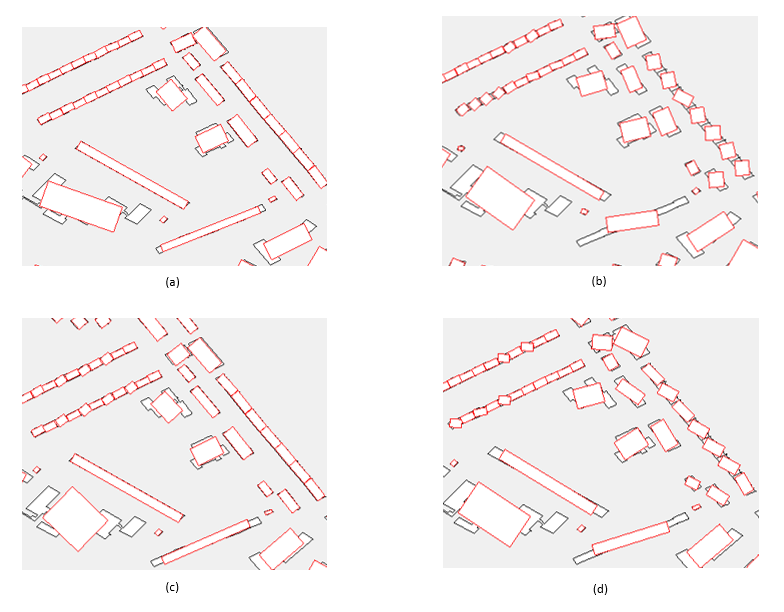
\includegraphics[width=17cm]{prosek_porovnani.png}
    \caption{Porovnání generalizačních algoritmů pro Prosek. Algoritmy: (a) \emph{MAER}, (b) \emph{Wall Average}, (c) \emph{Longest Edge} a (d) \emph{Weighted Bisector}. (vlastní zpracování).}
\end{figure}

\par Protože je většina budov datasetu obdélníkového tvaru, není na nich co generalizovat. Pro tyto tvary se jako nejvhodnější algoritmus pro určení hlavního směru budov opět jeví \textbf{\emph{MAER}}, který i nejpřesněji zachoval natočení jednotlivých budov. O něco méně přesný, avšak podobně úspěšný byl opět \textbf{\emph{Longest Edge}}, který měl problémy s navazujícími budovami v horní části výřezů. 
\par Algoritmy \textbf{\emph{Wall Average}} a \textbf{\emph{Weighted Bisector}} si s přesností vedly podobně. Oba tyto algoritmy nebyly schopny zachytit skutečný směr budov v navazující zástavbě, a to i přesto, že jsou jenom obdélníkového tvaru. V případě nekonvexního půdorysu základní školy (ve výřezech dole vlevo) však nejpřesněji vystihly jeho orientaci a vedly si lépe než MAER a Longest Edge.

\section*{Dataset Chotěboř}

\par Vybraná část města Chotěboř obsahuje především domovou zástavbu, která na sebe příliš nenavazuje. Jednotlivé půdorysy jsou primárně obdélníkového nebo čtvercového tvaru (\emph{Obrázek 14}). V horní části datasetu (není ve výřezech) je domov důchodců ve tvaru písmena L. Tento tvar mají i některé další půdorysy domů. 

\begin{figure}[h]
\centering
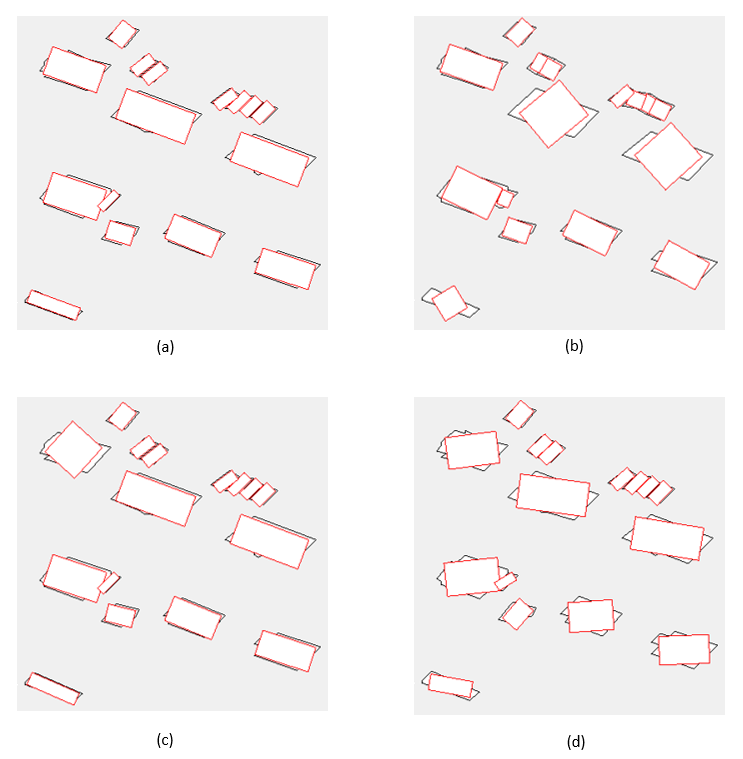
\includegraphics[width=17cm]{chotebor_porovnani.png}
    \caption{Porovnání generalizačních algoritmů pro Chotěboř. Algoritmy: (a) \emph{MAER}, (b) \emph{Wall Average}, (c) \emph{Longest Edge} a (d) \emph{Weighted Bisector}.  (vlastní zpracování).}
\end{figure}

\par Protože jsou tvary půdorysů opět především pravidelné, konfiguraci obdélníkových budov nejpřesněji detekovaly \textbf{\emph{MAER}} a \textbf{\emph{Longest Edge}} s téměř stejnými výsledky. 
\par U algoritmu \textbf{\emph{Wall Average}} již došlo k nesprávnému odhadu hlavního směru některých větších budov, avšak přibližně zachovává jejich původní tvar. Algoritmus \textbf{\emph{Weighted Bisector}} fungoval uspokojivě při obdélníkových budovách. O něco komplikovanější tvary však již nenatočil správně a z tohoto hlediska si vedl hůře než ostatní algoritmy.
\par Budovu domovu důchodců ani jeden algoritmus nedokázal adekvátně generalizovat pro její tvar. Půdorys ve tvaru písmena L byl ve všech případech nahrazen téměř čtvercovým obdélníkem.

\par V tabulce 1 je vyhodnocena relativní přesnost jednotlivých algoritmů.

\begin{table}[htbp]
    \centering
    \caption{ Úspěšnost jednotlivých algoritmů v \%}
    \begin{tabular}{|l||c||c||c||c|} 
     \hline\large
         \textbf{Algoritmus} & \textbf{Vinohrady} & \textbf{Prosek} & \textbf{Chotěboř} & \textbf{ průměr }\\ %[0.5ex] 
             \hline\hline
             \emph{\small MAER} & \small 92 &\small 90 & \small 95 & \small 92,3 \\
             \hline
             \emph{\small Wall Average} & \small 87 &\small 78 & \small 89 & \small 84,6 \\
             \hline
             \emph{\small Longest Edge} & \small 95 &\small 83 & \small 91 & \small 89,6 \\
             \hline
             \emph{\small Weighted B.} & \small 55 &\small 70 & \small 80 & \small 68,3 \\
             \hline
    \end{tabular}
\end{table}

\section*{Shrnutí}

\par Pro vybrané datasety se jako nejvhodnější algoritmus pro určení hlavního směru budovy jeví \textbf{\emph{Minimum Area Enclosing Rectangle}} (toto tvrzení potvrzuje i Tabulka 1), pak \textbf{\emph{Longest Edge}}. Nejméně uspokojivé výsledky dosahoval algoritmus \textbf{\emph{Weighted Bisector}}, který si však v několika případech dokázal lépe poradit s nekonvexními půdorysy. Algoritmus \textbf{\emph{Wall Average}} dosahoval různé úspěšnosti. Ve vlastní implementaci tohoto algoritmu se pracuje s aritmetickým průměrem zbytků úhlů a bylo by vhodné porovnat tyto výsledky s verzí, která pracuje s váženým průměrem zbytků.